To understand if the solution works it will be subjected to tests with origin in the requirement specification in section \ref{sec:reqspec}. The requirements, which will be tested, are listed here:

\begin{enumerate}
\setlength{\itemsep}{0mm}
	\item Detect position of table.
	\item Detect position of balls.
	\item Identify balls with high accuracy.
	\item Position and identification of balls should be obtained within one second
	\item Work with mixed light conditions and not only those stated in WPAB rules \ref{sec:rules}.
\end{enumerate}

The tests for the first four requirements will be done individually with the different lighting as described in section \ref{sec:testsetup}. The fifth requirement will be tested within the other requirements by altering the light.

\section{Test setup}
\label{sec:testsetup}
The test were conducted in the multimedia lab located in room A6-314 on Niels Jernes Vej 12 in Aalborg where image and video material for the solution to this project were made. 

%A second smaller test, to illustrate that the solution will work for different pool tables, is conducted in the DE-Klub which is a student bar located in A4-101 at Frederik Bajers Vej 7 in Aalborg. 
The pool table can be seen in figure \ref{fig:pooltableimg}. The videos used for the test can be found \fixme{indsæt ref}

\begin{figure}[H]
\begin{center}
\leavevmode
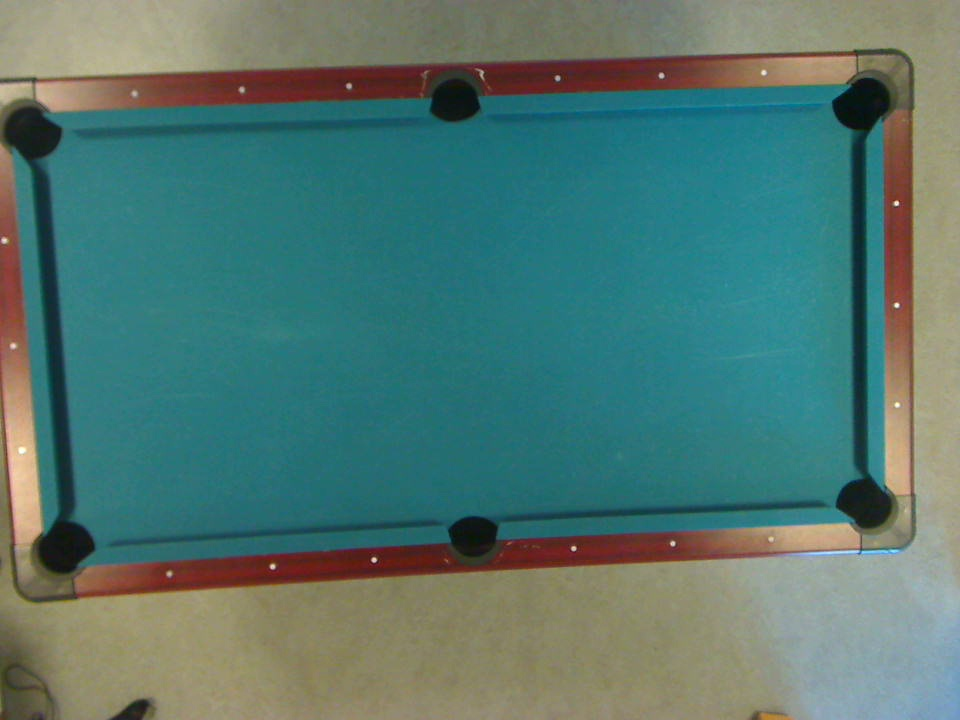
\includegraphics[width=0.4\textwidth]{images/test/light/input}
\end{center}
   \caption{The pool table used for testing.}
  \label{fig:pooltableimg}
\end{figure} 

The tests were made in two light conditions: normal and mixed. These conditions can be seen in figure \ref{fig:difflightcon}.

\begin{figure}[H]
  \centering
  \subfloat[Normal illumination]{\label{fig:gull}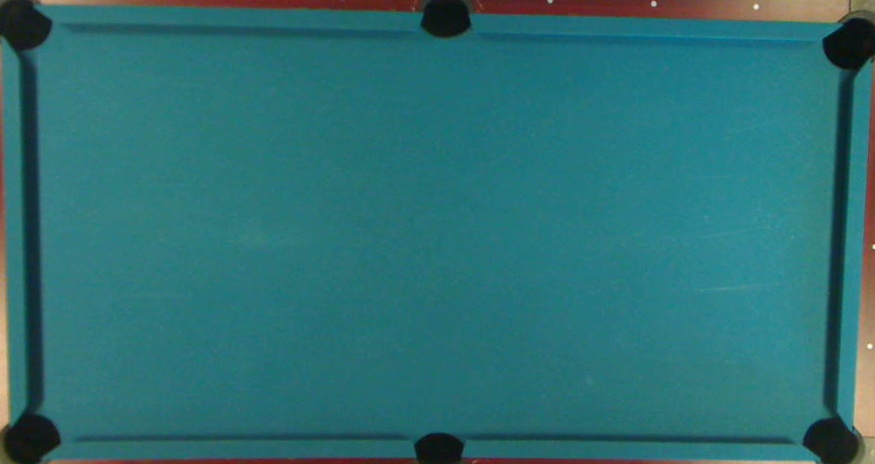
\includegraphics[width=0.48\textwidth]{images/test/light/detectedtable}}
  \quad           
  \subfloat[Mixed illumination]{\label{fig:tiger}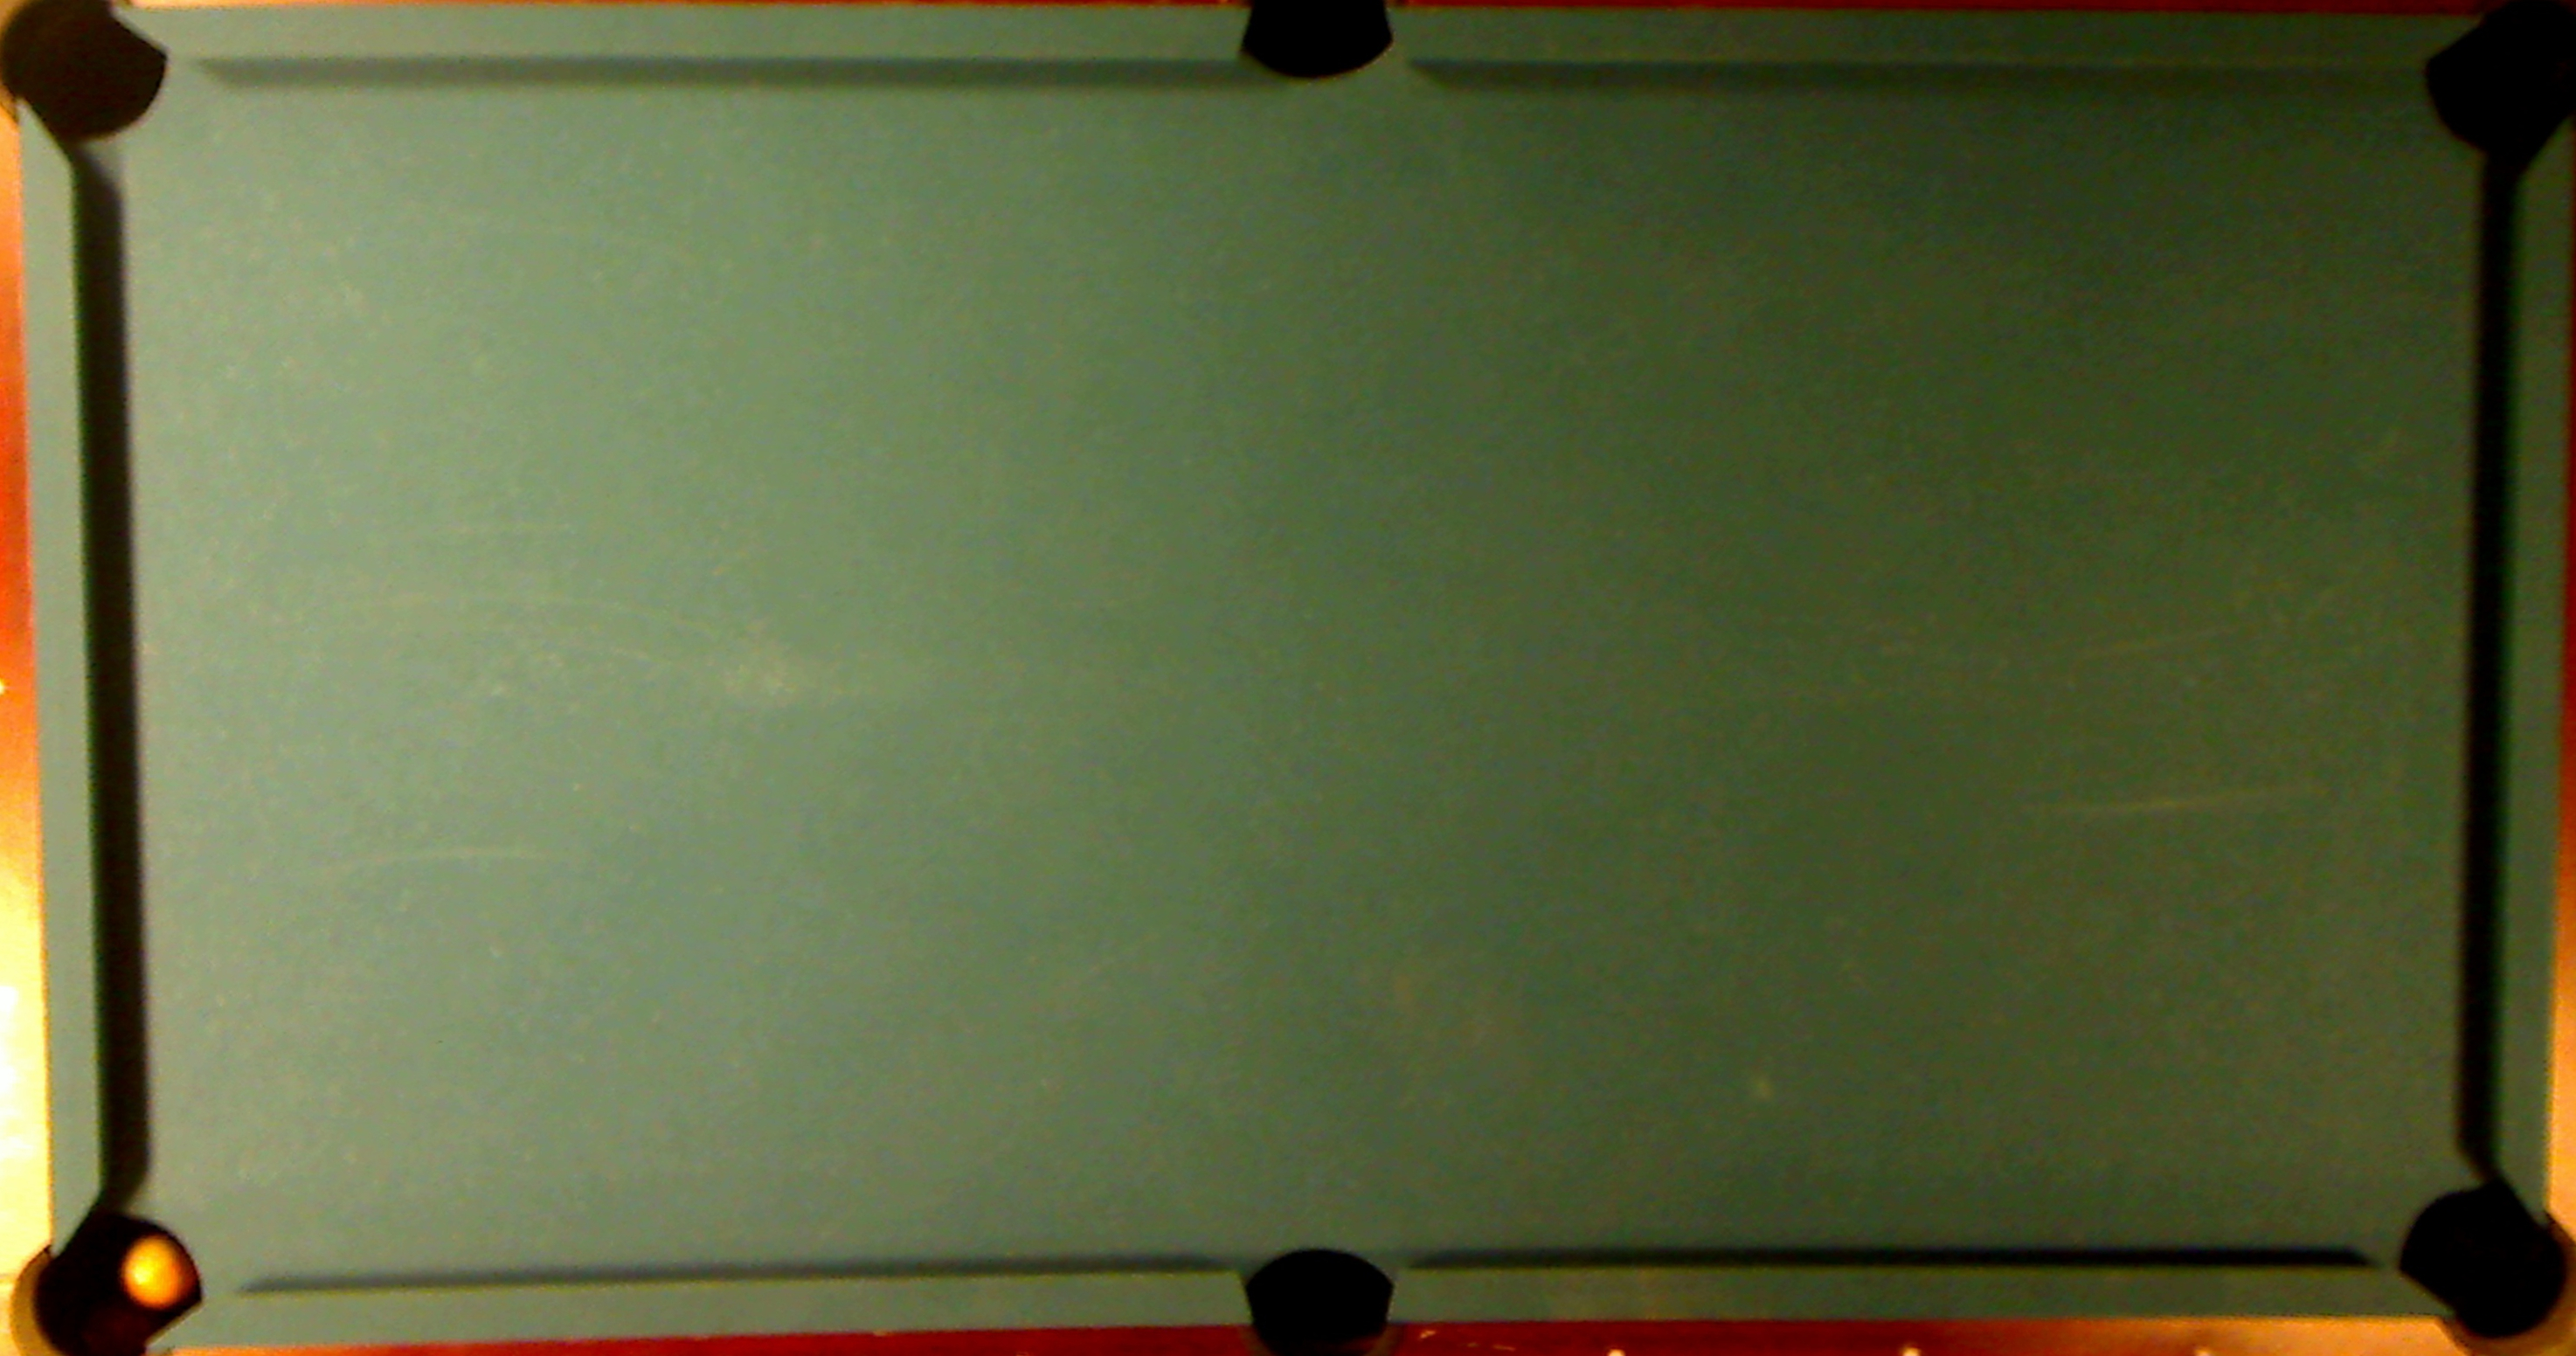
\includegraphics[width=0.48\textwidth]{images/test/mixed/detectedtable}}
   \caption{Table cloth in the two different light conditions.}
  \label{fig:difflightcon}
\end{figure}


\section{1) Detect position of table}

This was tested numerous times and if the position of the table is within the view of the camera the table will be found in both light conditions.

\section{2) Detect position of balls}
The precision of the ball positions is important, since the identification relies on having the correct positions. To test the detection, the balls have been positioned in different scenarios to test for different kinds of weaknesses in the detector. The following scenarios has been tested:
\begin{enumerate}
	\item Balls laying apart.
	\item Balls clustered by color
	\item Balls laying in start position as described in section \ref{sec:rules}.
\end{enumerate}
In some of the tests, two results have been recorded. One representing the best case scenario and one representing the worst case scenario. This is done to illustrate the differences observed during the test.

\subsection{Balls laying apart}
The least difficult test for the detection of balls is where the balls are laying apart. The result of the test with normal light can be seen in figure \ref{fig:apartnormal} and for the mixed light in figure \ref{fig:apartmixed}.

\begin{figure}[htpb]
  \centering
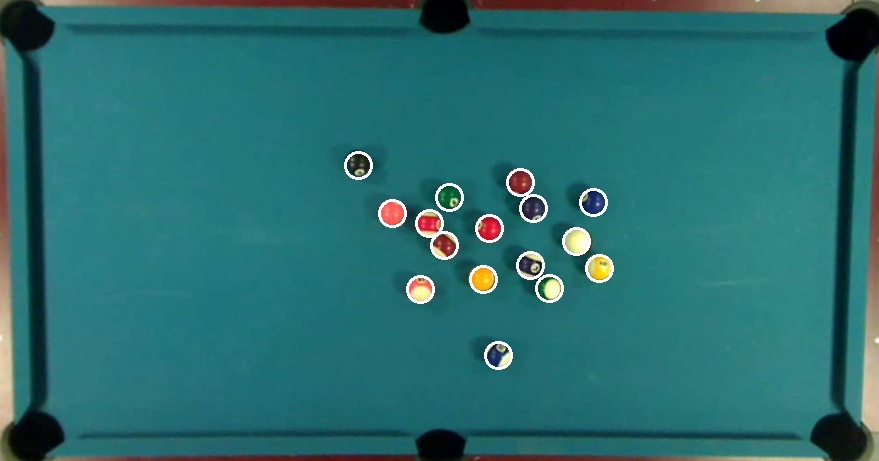
\includegraphics[width=0.5\textwidth]{images/test/light1/laying-apart}
   \caption{Balls laying apart - normal light.}
  \label{fig:apartnormal}
\end{figure}

\begin{figure}[htpb]
  \centering
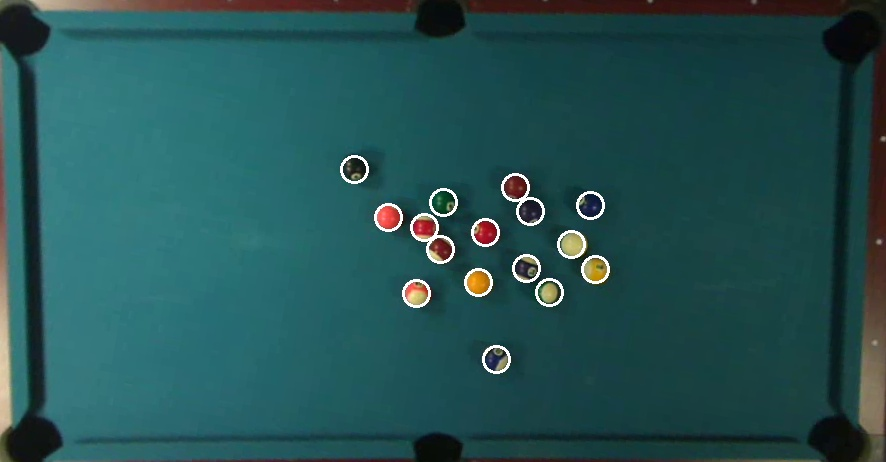
\includegraphics[width=0.5\textwidth]{images/test/mixed1/laying-apart}
   \caption{Balls laying apart - mixed light.}
  \label{fig:apartmixed}
\end{figure}

There is no significant change in the behavior of the system between the mixed, and the normal lighting. The balls are detected correctly in both the left and the right side of the table. This shows that the detection is adaptive towards change in lighting across the table in an uncluttered ball arrangement.

\subsection{Balls clustered by color}
As mentioned in section \ref{sec:balls-locate}, the ball detection works by finding areas that minimizes the color variance. To test for weaknesses in this method, the scenario seen in figures \ref{fig:clustersnormal} and \ref{fig:clustersmixed} is tested.
\begin{figure}[htpb]
  \centering
  \subfloat[Black ball low precision]{\label{fig:gull}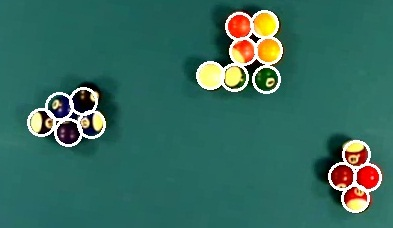
\includegraphics[width=0.4\textwidth]{images/test/light1/clusters-1}}
  \quad
   \subfloat[Two balls detected wrong]{\label{fig:tiger}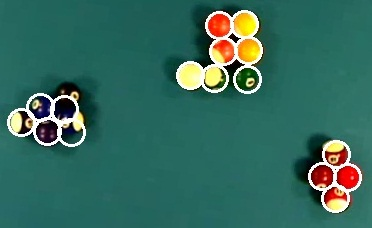
\includegraphics[width=0.4\textwidth]{images/test/light1/clusters-2}}
	\quad
   \caption{Balls in clusters - normal light.}
  \label{fig:clustersnormal}
\end{figure}

\begin{figure}[htpb]
  \centering
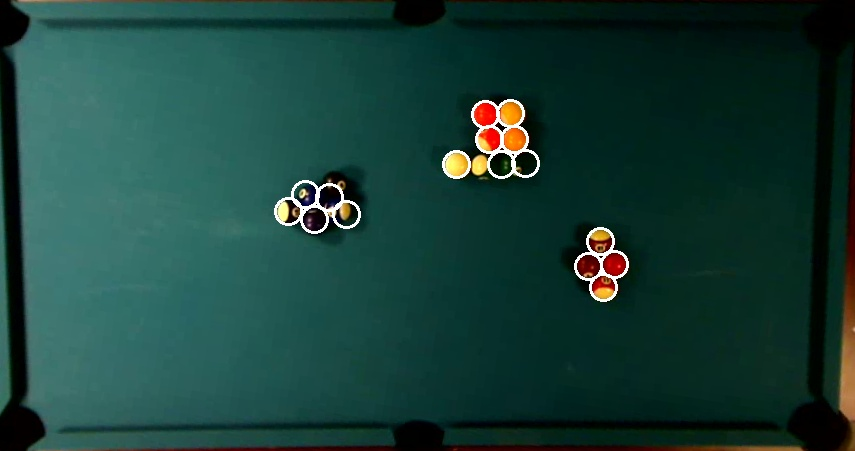
\includegraphics[width=0.5\textwidth]{images/test/mixed1/clusters-2}
   \caption{Balls in clusters - mixed light. Several detection problems.}
  \label{fig:clustersmixed}
\end{figure}
The balls are not correctly detected in this scenario. The problem is most significant in the left cluster that consists of the dark colored balls: purple, blue and black. The problem worsens when the image is darker in figure \ref{fig:clustersmixed}. The detection of the red colored balls does however not result in any errors or positional problems. 


\subsection{Balls laying in start position}
The balls are placed in the start position with all balls except the cue ball clustered. This is the most difficult condition to test positions of the pool balls. The test was done while the balls were laying still and the result of the test with normal light can be seen in figure \ref{fig:poolposstart} and for the mixed light in figure \ref{fig:poolposstart2}.

\begin{figure}[htpb]
  \centering
   \subfloat[Correct detection]{\label{fig:poolposstart-good}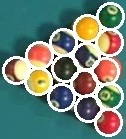
\includegraphics[width=0.2\textwidth]{images/test/light1/start-normal-1}}
\quad
   \subfloat[Incorrect detection]{\label{fig:poolposstart-bad}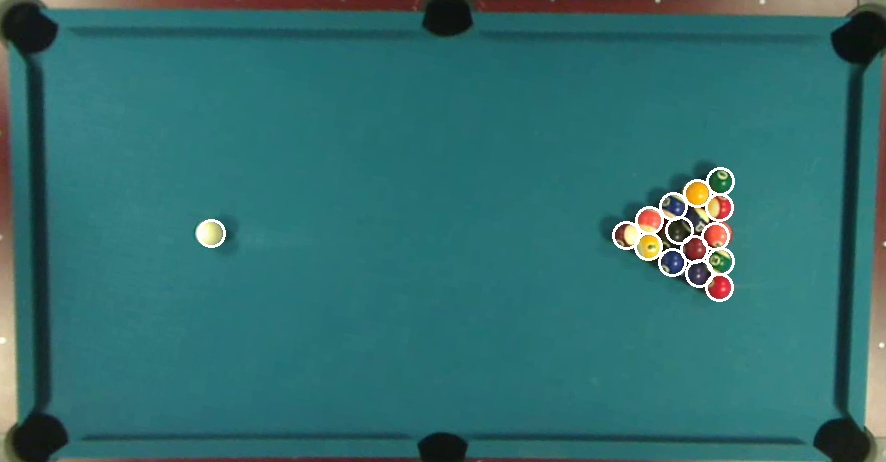
\includegraphics[width=0.2\textwidth]{images/test/light1/start-normal-2}}
   \caption{Balls in start position - normal light.}
  \label{fig:poolposstart}
\end{figure}

\begin{figure}[htpb]
  \centering
  \subfloat[Correct detection]{\label{fig:gull}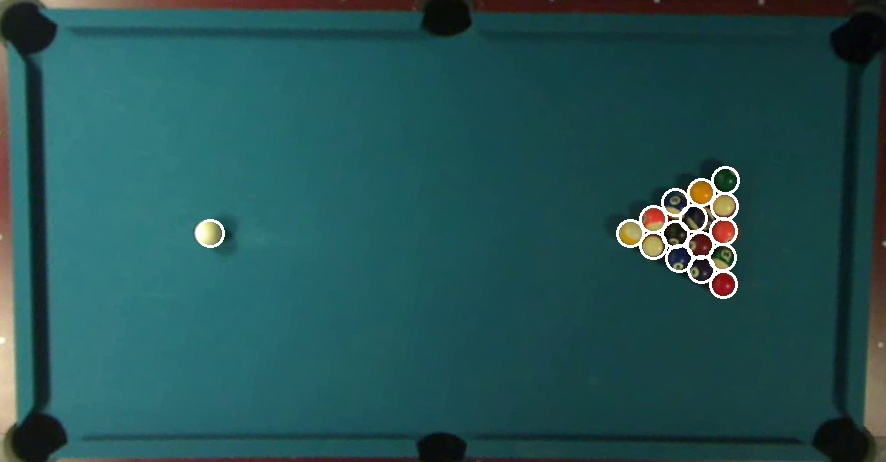
\includegraphics[width=0.2\textwidth]{images/test/mixed1/start-mixed-1}}
\quad
   \subfloat[Incorrect detection]{\label{fig:tiger}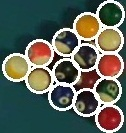
\includegraphics[width=0.2\textwidth]{images/test/mixed1/start-mixed-2}}
\quad
   \caption{Balls in start position - mixed light.}
  \label{fig:poolposstart2}
\end{figure}

The system performs almost equally in the light environment seen in figure \ref{fig:poolposstart} as in mixed lighting in figure \ref{fig:poolposstart2}. For the system to find all positions in this situation, it is important that the positions of the first detected balls are correct, because their positions will affect the rest of the detection as mentioned in section \ref{sec:balls-locate}. Problems arise in a situation like the one seen in figure \ref{fig:poolposstart-bad}. The black and orange balls have been inaccurately detected, and the consequence is that there is insufficient room to detect the striped purple 14.


\section{Identify balls with high accuracy}
The identification of the balls is done by first calibrating the system with the colors of the balls. Afterwards testing the identification with the balls placed in two different scenarios:

\begin{enumerate}
\setlength{\itemsep}{0mm}
	\item With \textbf{Minimum} white area visible
	\item With \textbf{Maximum} white area visible
\end{enumerate}
This is done to test the borderline cases for when a ball is considered solid, striped or white.

\subsection{With minimum white area visible}
This scenario will test if the identifier has problems that causes striped balls to be identified as solid balls.
The result of the test with normal light can be seen in figure \ref{fig:minnormal} and for the mixed light in figure \ref{fig:minmixed}.
\begin{figure}[htpb]
  \centering
  \subfloat[Input image]{\label{fig:gull}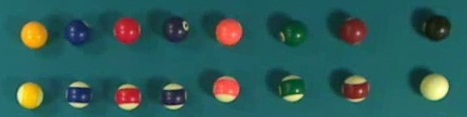
\includegraphics[width=0.5\textwidth]{images/test/light1/min-white-input}}
  \quad
   \subfloat[Found balls]{\label{fig:tiger}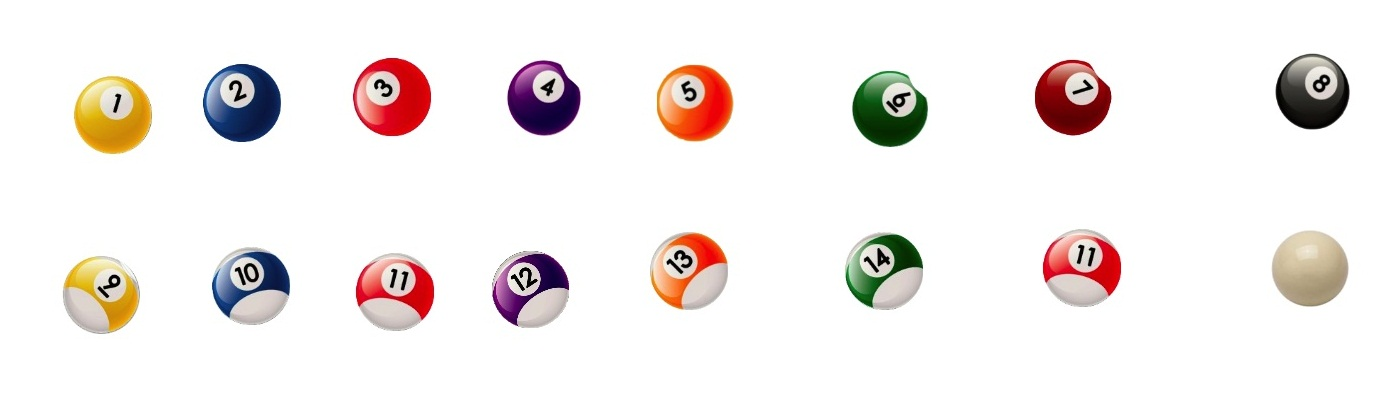
\includegraphics[width=0.5\textwidth]{images/test/light1/min-white-output}}
	\quad
   \caption{Balls having minimum white area visible - normal light.}
  \label{fig:minnormal}
\end{figure}

\begin{figure}[htpb]
  \centering
  \subfloat[Input image]{\label{fig:gull}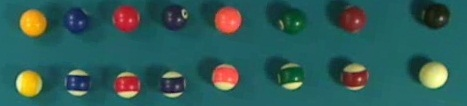
\includegraphics[width=0.5\textwidth]{images/test/mixed1/min-white-input}}
  \quad
  \subfloat[Found balls]{\label{fig:tiger}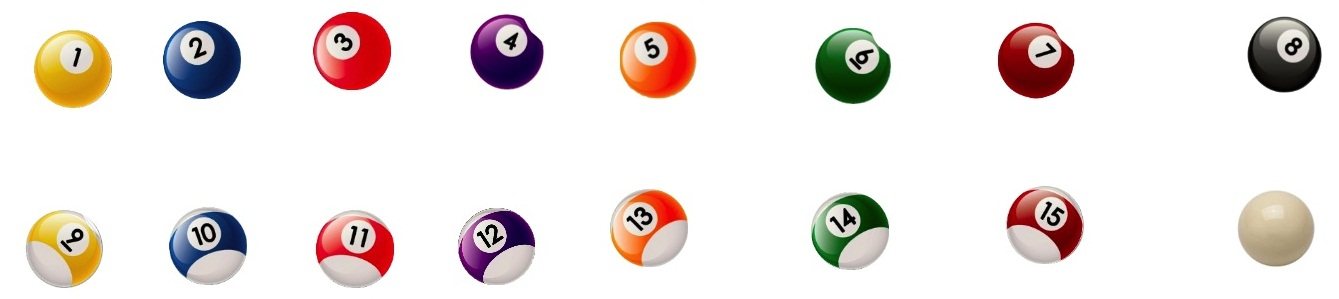
\includegraphics[width=0.5\textwidth]{images/test/mixed1/min-white-output}}
  \quad
   \caption{Balls having minimum white area visible - mixed light.}
  \label{fig:minmixed}
\end{figure}
All balls on both mixed and normal lighting are correctly identified, except for striped brown 15 which has been classified as red striped 11. This occurs because of the colors begin close. None of the striped balls are misclassified as solids, independent of lighting conditions.

\subsection{With maximum white area visible}
This test will illustrate if the ratio of white pixels is defined well enough to identify if the ball is solid or striped. Also the detection of correct colors will be tested. The result of the test with normal light can be seen in figure \ref{fig:maxnormal} and for the mixed light in figure \ref{fig:maxmixed}.

\begin{figure}[htpb]
  \centering
  \subfloat[Input image]{\label{fig:gull}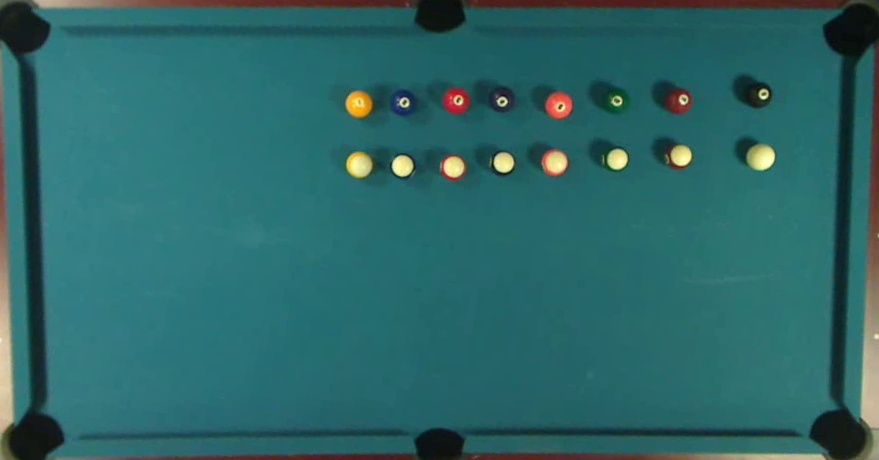
\includegraphics[width=0.5\textwidth]{images/test/light1/max-white-input}}
  \quad
   \subfloat[Found balls]{\label{fig:tiger}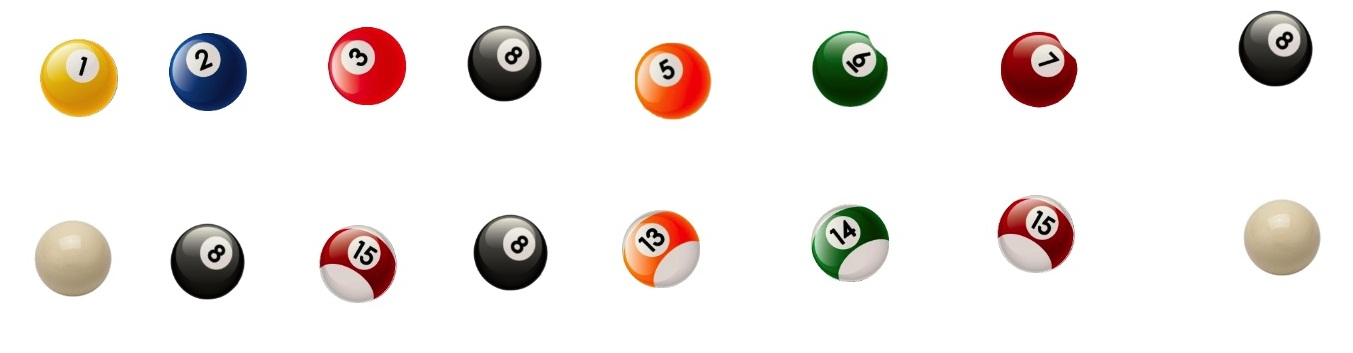
\includegraphics[width=0.5\textwidth]{images/test/light1/max-white-output}}
	\quad
   \caption{Balls having maximum white area visible - normal light.}
  \label{fig:maxnormal}
\end{figure}

\begin{figure}[htpb]
  \centering
  \subfloat[Input image]{\label{fig:gull}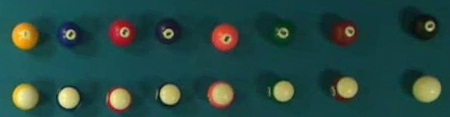
\includegraphics[width=0.5\textwidth]{images/test/mixed1/max-white-input}}
  \quad
  \subfloat[Found balls]{\label{fig:tiger}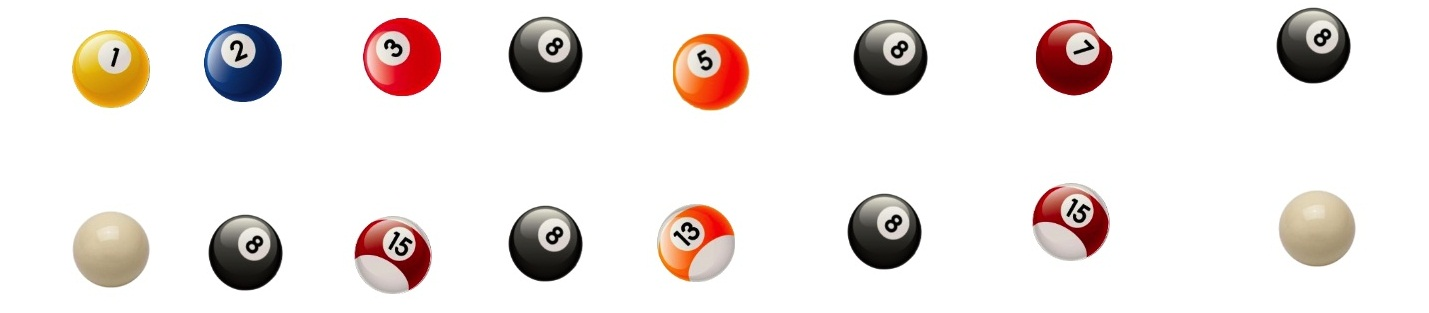
\includegraphics[width=0.5\textwidth]{images/test/mixed1/max-white-output}}
  \quad
   \caption{Balls having maximum white area visible - mixed light.}
  \label{fig:maxmixed}
\end{figure}
The identification fails in both normal and mixed light. Identification of the striped balls in this scenario is problematic due to the small amount of color available. Most of the striped balls are however, identified as being striped in spite of the small amount of color. In the mixed light environment, several of the balls are identified as being the black 8-ball which is caused by the identifier being sensitive to the change in lighting.

\subsection{Position and identification of balls should be obtained within one second}
The system speed was tested with different sizes of video and image input from the used webcam. It is able to find the position and identify the balls within one second. This test was done on a Core-Duo L2400 running at 1.67 Ghz. 
